
\section{An expected $3$ approximation for correlation clustering}

	\begin{align}
		\min \qquad \sum_{i \in F, j \in C}x_{i, j} d^q(i, j) \tag{$\text{LP}_{\text{strong}}$} \qquad  \label{LP:strong}
	\text{s.t.} \\
		y_i &= 1 & & \forall i \in S_0 &\label{LPs:S0}\\
		 x_{i,j} &= 0 & &\forall i, j \, \text { s.t } \, d(i,j) >  R_j & \label{LPs:R} \\
	    \sum_{j} d^q(i,j) x_{i,j} & \leq \rho \tilde U y_i & & \forall i \notin S_0 & \label{LPs:star} \\[-6pt]
	    x_{i,j} &= 0 & &\forall i \notin S_0, j \, \text { s.t } \, d^q(i,j) >  \rho \tilde U &\label{LPs:R-d}
	\end{align}




\begin{algorithm}
\caption{{\sf Dynamic}$(e_\bt, \pm)$}
\label{alg:dynamicf}
\begin{algorithmic}[1]
\If{the operation $\sigma_\bt$ is $(e_\bt, +)$}
%%\State \mysp {\bf If} there is a set $S$ in $\St$ which contains $e_t$, assign $e_t$ to this set
\State  Set $\levelt(e) = \max_{S:e \in S} \levelt(S)$, and define $\yt(e)$ to be $\frac{1}{2^{\levelt(e)}}$.
\State  For all sets $S$ containing $e$
\State \spc Update $\yt(S) \leftarrow \yt(S) + \yt(e)$.
\State \spc Add $e$ to the appropriate list in $\lists(S)$, and build $\nodelist(e)$.
\State\spc  If $\yt(S) > \beta  c_S$, and $S$ is already not in $Q$, add it to $Q$.
\ElsIf{the operation $\sigma_\bt$ is $(e_\bt, -)$}
\State For all sets $S$ containing $e$ (traverse using $\nodelist(e)$)
\State  \spc Update $\yt(S) \leftarrow \yt(S) - \yt(e)$.
\State \spc Delete  $\nodelist(e)$ and all $\node(e,S)$.
\State \spc If $\yt(S) < \frac{c_S}{\beta}$, and $\levelt(S) > b_S$ and $S$ is not in $Q$, add $S$ to $Q$.
\EndIf
\State If $Q$ is non-empty, call \FIX.
\end{algorithmic}
%\end{center}
\end{algorithm}




We first describe the algorithm (Algorithm \ref{alg:CC:3apx}) [{\color{red} Aggregating Inconsistent Information: Ranking and Clustering, Nir Ailon, Moses Charikar, Alantha Newman}]:

\begin{algorithm}[$3$ approximation for correlation clustering] \label{alg:CC:3apx}
\begin{enumerate}
    \item Pick any point $v$ uniformly randomly.
    \item Form a cluster $C$ composed of $v$ with all points that share a $+$ edge with $v$.
    \item Remove $C$ from $V$ and recurse on the induced subgraph $V \setminus C$.
\end{enumerate}
\end{algorithm}

We set up the analysis as follows: we construct a graph $G$ where two vertices are connected by an edge if they share a positive edge and are disconnected if they share a negative edge. If two vertices $u$ and $v$ are true twins (they share the same set of neighbors in $V \setminus \{ u,v \}$) then Algorithm \ref{alg:CC:3apx} will not wrongly classify the edge $u,v$.\\

\noindent The number of mistakes made by the algorithm can be accounted as follows. In any iteration, let $V'$ denote the set of remaining (unclustered) vertices. Then, the number of mistakes made by forming a cluster $C$ centered at $u$ is equal to the number of points that form a triangle with $u$ having two positive and one negative edge in the induced subgraph on $V'$. This is because the remaining mistakes made by $C$ with previously clustered points are already accounted in the previous iterations.\\

\noindent Let us use $t$ to denote the triple $(u,v,w)$ where $\Delta uvw$ forms a bad triangle with two positive edges and one negative edge. Let $A_t^{(i)}$ denote the event that in iteration $i$, one of $u,v,w$ is chosen as a pivot and that $u,v,w$ belong to $V'$ in this recursive call of the algorithm. The total cost of the algorithm is then $\sum_i \sum_t \mathbbm{1} (A_t^{(i)})$ which is equal to $\sum_t A_t$ where $A_t$ denotes the event that one of $u,v,w$ is chosen as a pivot and that $u,v,w$ belong to $V'$ in the same recursive call of the algorithm.\\

\noindent Therefore, the expected cost of the algorithm is $\sum_t p_t$ where $p_t$ is the probability of $A_t$ occurring.\\

    \noindent Observe that any algorithm will have to pay a unit cost for each triangle among any set of edge disjoint triangles from $B$. Therefore, we construct an optimization problem that finds the maximum number of edge disjoint triangles from $B$ and conclude that the cost of $OPT$ is at least this much. Let $B$ denote the set of tuples $(u,v,w)$ corresponding to bad triangles $\Delta uvw$. We therefore consider the dual to a relaxed LP,

\begin{alignat}{3} \label{LP:CC-relax-dual}
		&\text{Find: } && \argmax\ \sum_{t \in B} z_t, \nonumber\\
		&\text{Subject to:} \quad && \forall e = (u,v) \in E ,\ \sum_{t \in B : u,v \in t} z_t \le 1, \nonumber\\
		& && \forall t \in B,\ z_{t} \in [ 0,1 ].\tag{LP1}
\end{alignat}

We now show that the set of probabilities $\{ p_t / 3,\ t \in B \}$ forms a valid solution to this LP. This proves that the algorithm is $3$ approximate since any solution to \ref{LP:CC-relax-dual} is a lower bound to $OPT$. Consider any edge $e = (u,v)$ and the bad triangles $B_{uv} = \{ t_w : (u,v,w) \in B \}$ it is part of. For any of these bad triangles, if the third vertex $w$ is picked as a cluster center then $(u,v)$ will become misclassified. The probability that $w$ is picked conditioned on $A_{t_w}$ is $1/3$. Therefore, we have:
\begin{equation} \label{eq:0000}
    P ( (u,v) \text{ is misclassified}) = \sum_{t \in B_{uv}} \frac{1}{3} p_t.
\end{equation}
Therefore, for every edge $e = (u,v)$, $\sum_{t \in B_{uv}} \frac{1}{3} p_t \le 1$ and this forms a feasible fractional solution to \ref{LP:CC-relax-dual}.

\begin{figure}[ht]
\centering
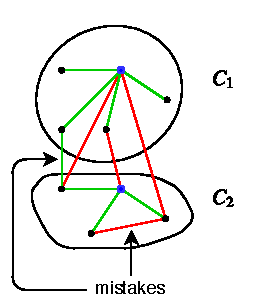
\includegraphics{./img/3apx.pdf}
\caption{An instance of Algorithm \ref{alg:CC:3apx}}
\label{fig:5}
\end{figure}

\section{Extending this idea to $m$-robust correlation clustering}

We first provide the algorithm:

Solve \ref{IP:CC4} (relaxation) optimally. Let the fractional solution be denoted $\{ x_{uv}  \}$. Remove those vertices with $Y_u^* \ge 1/4$. Perform the Algorithm  \ref{alg:CC:3apx} clustering on the remaining vertices.

Any solution to the problem must pay a cost of $1$ for every edge-disjoint set of triangles that does not have any vertex removed. Therefore, consider the following relaxed LP:

\begin{alignat}{3} \label{LP:CC-relax:2}
		&\text{Find: } && \argmin\ \sum_{(u,v) \in \binom{V}{2}} x_{uv}, \nonumber\\
		&\text{Subject to:} \quad && \forall t = (u,v,w) \in B ,\ Y_u + Y_v + Y_w + x_{uv} + x_{vw} + x_{uw} \ge 1, \nonumber\\
		& && \sum_{u} Y_u \le m \nonumber\\
		& && \forall (u,v) \in \binom{V}{2},\ x_{uv} \in [ 0,1 ] \nonumber\\
		& && \forall u \in V,\ Y_u \in [0,1]. \tag{LP3}
\end{alignat}

According to our algorithm, we round the $Y_u^* \ge 1/4$ to $1$ and $Y_u^* \le 1/4$ to $0$. Therefore, we do not exceed the budget of number of vertices to remove by more than a factor of $4$. On the other hand, for any vertex that is removed, the corresponding bad triangles do not incur any cost for the algorithm. In case, none of the vertices of the triangle are removed, the constraints of \ref{LP:CC-relax:2} are now represented as:
\begin{alignat}{3} \label{LP:CC-relax-reduced:2}
		&\text{Find: } && \argmin\ \sum_{(u,v) \in \binom{V}{2} : Y_u^*, Y_v^* \le 1/4} x_{uv}, \nonumber\\
		&\text{Subject to:} \quad && \forall t = (u,v,w) \in B : Y_u^* \ \&\ Y_v^* \ \&\ Y_w^* \le 1/4,\quad x_{uv} + x_{vw} + x_{uw} \ge 1/4, \nonumber\\
		& && \forall (u,v) \in \binom{V}{2},\ x_{uv} \in [ 0,1 ]. \tag{LP4}
\end{alignat}
Let $B'$ represent the set of triples $(u,v,w)$ in $B$ such that $Y_u^* \ \&\ Y_v^* \ \&\ Y_w^* \le 1/4$.
The dual of this LP is:
\begin{alignat}{3} \label{LP:CC-relax-reduced-dual:2}
		&\text{Find: } && \argmax\ \frac{1}{4} \sum_{t \in B'} z_t, \nonumber\\
		&\text{Subject to:} \quad && \forall e = (u,v) \in E ,\ \sum_{t \in B' : u,v \in t} z_t \le 1, \nonumber\\
		& && \forall t \in B',\ z_{t} \in [ 0,1 ].\tag{LP5}
\end{alignat}
By a similar logic as previously, the solution $\{ \frac{1}{3} p_t, t \in B'\}$ is a valid solution to the dual, having cost equal to $\frac{1}{12} \sum_{t \in B'} p_t$. The algorithm has an expected cost of $\sum_{t \in B'} p_t$. This is because the algorithm only accumulates the cost corresponding to the event $A_t$ if none of the vertices in $t$ are removed in the preliminary vertex removal stage.

$---------------------------------------------$

\section{A combinatorial algorithm for $m$-robust clustering on complete graphs?}

Let $OPT^*$ denote the optimal solution to \ref{LP:CC-relax:2}. Let us consider the following relaxation to \ref{LP:CC-relax:2},

\begin{alignat}{3} \label{LP:CC-relax:3}
		&\text{Find: } && \argmin\ \sum_{(u,v) \in \binom{V}{2}} x_{uv} + \frac{OPT^*}{m} \sum_u Y_u, \nonumber\\
		&\text{Subject to:} \quad && \forall t = (u,v,w) \in B ,\ Y_u + Y_v + Y_w + x_{uv} + x_{vw} + x_{uw} \ge 1, \nonumber\\
		& && \forall (u,v) \in \binom{V}{2},\ x_{uv} \in [ 0,1 ] \nonumber\\
		& && \forall u \in V,\ Y_u \in [0,1]. \tag{LP6}
\end{alignat}

\noindent We know that the optimal solution to \ref{LP:CC-relax:3} is within a factor of $2$ of the optimal solution to \ref{LP:CC-relax:2}. This is because the the optimal solution of \ref{LP:CC-relax:2} is a feasible solution to \ref{LP:CC-relax:3} with a cost of $2 OPT^*$. The dual of \ref{LP:CC-relax:3} is:

\begin{alignat}{3} \label{LP:CC-relax-dual:3}
		&\text{Find: } && \argmax\ \sum_{t \in B} z_t, \nonumber\\
		&\text{Subject to:} \quad && \forall u,v \in \binom{V}{2},\ \sum_{t : u,v \in t} z_t \le 1, \nonumber\\
		& && \forall v \in V,\ \sum_{t : u \in t} z_t \le \frac{OPT^*}{m} \nonumber\\
		& && \forall t \in B,\ z_t \ge 0. \tag{LP7}
\end{alignat}

\begin{algorithm} \label{alg:IP:CC7}
Run Charikar clustering. Delete vertices which are connected to at least $OPT^* / m$ mis-classified edges.
\end{algorithm}

\begin{theorem}
This algorithm is a $(9,6)$ bi-criteria approximation for $m$-robust correlation clustering.
\end{theorem}
\noindent For brevity, let the function $\mathrm{Mis} (v)$ count the number of mis-classified edges associated with vertex $v$ in a clustering. After using Charikar's clustering, the expected number of mis-classified edges vertex $u$ is connected to is equal to, 
\begin{align} 
    \mathbb{E} [\mathrm{Mis} (u)] &= \sum_{v \ne u} P( (u,v) \text{ is misclassified})\\
    &= \sum_{v \ne u} \sum_{t : u,v \in t} p_t \qquad [\text{from Equation } \eqref{eq:0000}] \nonumber\\
    &= \sum_{t : u \in t} p_t. \label{eq:00004}
\end{align}
Using Markov's inequality, the probability that the vertex is deleted in the next round is:
\begin{align*}
    P (u \text{ is deleted}) &= P \left( \mathrm{Mis} (u) \ge \frac{OPT^*}{m} \right) \\
    &\le \frac{m}{OPT^*} \cdot \mathbb{E} [\mathrm{Mis} (u)]
\end{align*}
Therefore, the expected number of deleted vertices is:
\begin{align}
    \mathbb{E} [\# \text{ deleted vertices}] &\le \sum_u \frac{m}{OPT^*} \mathbb{E} [\mathrm{Mis} (u)] \nonumber\\
    &= \frac{m}{OPT^*} \sum_u \underbrace{\sum_{t : u \in t} p_t}_{\text{defined as } Z_u} \qquad [\text{ from Equation } \eqref{eq:00004} ] \nonumber\\
    &\le 3m \frac{\sum_t p_t}{OPT^*} \label{eq:0001}
\end{align}
The last inequality uses the fact that any $p_t$ may appear in at most $3$ different $Z_u$'s. Therefore, $\sum_u Z_u \le 3\sum_t p_t $. The RHS of Equation \eqref{eq:0001} is the ratio of Charikar's clustering to the optimal fractional solution of \ref{LP:CC-relax:2} which are known to be within a factor of $3$. Therefore,
\begin{equation*}
    \mathbb{E} [\# \text{ deleted vertices}] \le 9m
\end{equation*}
On the other hand, the expected cost of the algorithm is equal to:
\begin{equation} \label{eq:0003}
    ALG = \mathbb{E} \left[ \sum_{t : t \cap R = \phi} p_t \right],
\end{equation}
where $R$ is the random set of vertices that are connected to at least $OPT^* / m$ mis-classified edges. Every bad triangle $t$ that is counted in Equation \eqref{eq:0003} does not have more than $OPT^*/m$ mis-classified edges associated with each of its vertices. The cost in Equation \eqref{eq:0003} can be rewritten as,
\begin{equation}
    \mathbb{E} [ALG] = \sum_{t \in B} p'_t,
\end{equation}
where $p_t'$ is defined as $P \left( A_t \ \& \ \mathrm{Mis} (u) \le \frac{OPT^*}{m} \ \& \ \mathrm{Mis}(v) \le \frac{OPT^*}{m} \ \&\ \mathrm{Mis} (w) \le \frac{OPT^*}{m} \right)$, the probability that the cost of the bad triangle is counted after vertex deletion.
Consider the solution $ \mathbf{S}$ equal to $\{ p_t' / 3 : t \in B \}$. We show that this is a feasible solution to the relaxed dual \ref{LP:CC-relax-dual:3}. The edge constraints are satisfied by the same previous arguments since $p_t' \le p_t$. Consider any vertex constraint of \ref{LP:CC-relax-dual:3},
\begin{align*}
    \sum_{t : u \in t} z_t = \frac{1}{3} \sum_{t : u \in t} p_t'.
\end{align*}
This is equal to $1/3$ times the average number of mis-classified edges connected to $u$ after the vertex deletion stage (observe Equation \eqref{eq:00004} to understand) which itself cannot exceed $OPT^* / m$ (by the vertex deletion criterion).
Therefore, the cost of $\mathbf{S}$ lower bounds the optimal fractional solution of \ref{LP:CC-relax:3}. It is known that this does not exceed twice of $OPT^*$ which we benchmark our algorithm's cost against. Therefore, we have from \eqref{eq:0003} that,
\begin{align*}
    \frac{\mathbb{E} [ALG]}{OPT^*} \le 2 \frac{\mathbb{E} [ALG]}{OPT_{\ref{LP:CC-relax:3}}} &\le 2 \frac{\mathbb{E} [ALG]}{OPT_{\ref{LP:CC-relax-dual:3}}} \\
    &\le 2\frac{\mathbb{E} [ALG]}{\cost (\mathbf{S})} \\
    &= 6
\end{align*}